% Copyright (c) 2013 by the University of Waikato, Hamilton, NZ. 
% This work is made available under the terms of the 
% Creative Commons Attribution-ShareAlike 3.0 license, 
% http://creativecommons.org/licenses/by-sa/3.0/. 
%
% Version: $Revision$

\documentclass[a4paper]{book}

\usepackage{wrapfig}
\usepackage{graphicx}
\usepackage{hyperref}
\usepackage{multirow}
\usepackage{scalefnt}
\usepackage{tikz}

% watermark -- for draft stage
\usepackage[firstpage]{draftwatermark}
\SetWatermarkLightness{0.9}
\SetWatermarkScale{5}

% Copyright (c) 2009 by the University of Waikato, Hamilton, NZ. 
% This work is made available under the terms of the 
% Creative Commons Attribution-ShareAlike 3.0 license, 
% http://creativecommons.org/licenses/by-sa/3.0/. 
%
% Version: $Revision$

\newenvironment{tight_itemize}{
\begin{itemize}
  \setlength{\itemsep}{1pt}
  \setlength{\parskip}{0pt}
  \setlength{\parsep}{0pt}}{\end{itemize}
}

\newenvironment{tight_enumerate}{
\begin{enumerate}
  \setlength{\itemsep}{1pt}
  \setlength{\parskip}{0pt}
  \setlength{\parsep}{0pt}}{\end{enumerate}
}

% if you just need a simple heading
% Usage:
%   \heading{the text of the heading}
\newcommand{\heading}[1]{
  \vspace{0.3cm} \noindent \textbf{#1} \newline
}

\newcommand{\icon}[1]{\tikz[baseline=-3pt]\node[inner sep=0pt,outer sep=0pt]{\includegraphics[height=1.1em]{#1}};}


\title{
  \textbf{ADAMS} \\
  {\Large \textbf{A}dvanced \textbf{D}ata mining \textbf{A}nd \textbf{M}achine
  learning \textbf{S}ystem} \\
  {\Large Module: adams-timeseries} \\
  \vspace{1cm}
  
\includegraphics[width=2cm]{images/timeseries-module.png} \\
}
\author{
  Peter Reutemann
}

\setcounter{secnumdepth}{3}
\setcounter{tocdepth}{3}

\begin{document}

\begin{titlepage}
\maketitle

\thispagestyle{empty}
\center
\begin{table}[b]
	\begin{tabular}{c l l}
		\parbox[c][2cm]{2cm}{\copyright 2013} &
		\parbox[c][2cm]{5cm}{
\includegraphics[width=5cm]{images/coat_of_arms.pdf}} \\
	\end{tabular}
	
\includegraphics[width=12cm]{images/cc.png} \\
\end{table}

\end{titlepage}

\tableofcontents
\listoffigures
%\listoftables

%%%%%%%%%%%%%%%%%%%%%%%%%%%%%%%%%%%
\chapter{Introduction}
According to WikiPedia\footnote{\url{https://en.wikipedia.org/wiki/Time_series}{}}, 
a timeseries is \textit{is a sequence of data points, measured typically at 
successive points in time spaced at uniform time intervals.} ADAMS offers 
standalone tools, like the Timeseries Explorer, and flow components to loading,
processing and saving of timeseries data. Performing predictions using the 
Weka timeseries forecasting module, is possible as well. The following sections explain 
the available functionality in depth.

\begin{figure}[htb]
  \centering
  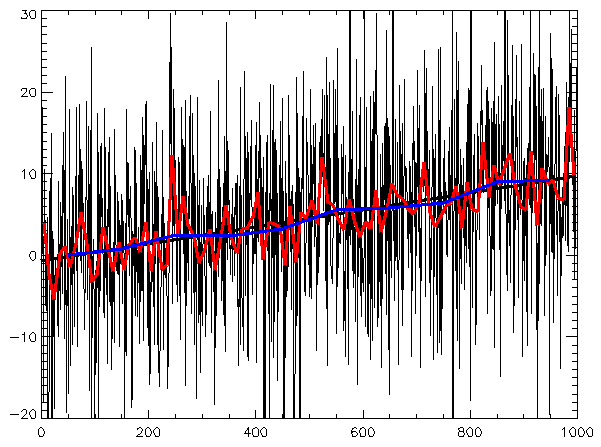
\includegraphics[width=10.0cm]{images/Random-data-plus-trend-r2.png}
  \caption{Image of random data plus trend, with best-fit line and different smoothings\cite{randomplot}.}
\end{figure}

%%%%%%%%%%%%%%%%%%%%%%%%%%%%%%%%%%%
\chapter{Flow}
The ADAMS flow allows you to comprehensively load, process and save timeseries
data, as well as make future predictions. \\

\noindent The following data conversions are available:
\begin{tight_itemize}
	\item \textit{SpreadSheetToTimeseries} -- generates a timeseries from two
	spreadsheet columns (timestamp and value).
	\item \textit{TimeseriesToArray} -- extracts the values of a timeseries to
	be further analyzed with array statistics, for instance.
	\item \textit{TimeseriesToSpreadSheet} -- turns a timeseries back into
	spreadsheet.
	\item \textit{TimeseriesToWekaInstances} -- generates data suitable for use
	with WEKA.
	\item \textit{WekaForecastContainerToArray} -- extracts the WEKA forecasts
	as an array for further processing.
	\item \textit{WekaForecastContainerToTimeseries} -- turns the WEKA forecasts
	into a proper timeseries data structure.\footnote{adams-timeseries-build\_and\_use\_forecaster2.flow}
	\item \textit{WekaInstancesToTimeseries} -- generates a timeseries from
	two attributes of a WEKA dataset (timestamp and value).\footnote{adams-timeseries-build\_and\_use\_forecaster2.flow}
\end{tight_itemize}

\noindent The following filters are available:
\begin{tight_itemize}
	\item \textit{Derivative} -- calculates a derivative from the timeseries 
	data.
	\item \textit{EquiDistance} -- ensures that the data points are evenly 
	spaced, can also interpolate to create timeseries with the same number of
	points.
	\item \textit{FastWavelet} -- applies a wavelet transform to a timeseries.
	\item \textit{LOWESS} -- applies LOWESS smoothing \cite{lowess}.
	\item \textit{Round} -- allows the rounding of the values associated with
	timestamps in the timeseries.
	\item \textit{SavitzkyGolay} -- transforms the timeseries using the
	Savitzky-Golay filter (smoothing and differentiation) \cite{savitzky}
	\item \textit{SetStart} -- shifts all data points relatively to a new 
	starting point for the timeseries.
	\item \textit{Window} -- extracts a specified window (or the inverse) from
	a timeseries.
\end{tight_itemize}

\noindent The following outlier detectors are available:
\begin{tight_itemize}
	\item \textit{MinPoints} -- requires the timeseries to have a certain 
	number (absolute or percentage) of values above a specified value.
\end{tight_itemize}

\noindent The following smoothers are available:
\begin{tight_itemize}
	\item \textit{LOWESSBased} -- uses a LOWESS filter for smoothing \cite{lowess}.
	\item \textit{SavitzkyGolayBased} -- uses the \textit{SavitzkyGolay} filter
	to smooth the timeseries.\cite{savitzky}
	\item \textit{SlidingWindow} -- wrapper smoother that applies the base 
	smoother to a sliding window.
\end{tight_itemize}

\noindent The following sources are available:
\begin{tight_itemize}
	\item \textit{TimeseriesDbReader} -- reads timeseries data from any
	JDBC database (required columns: ID, timestamp, value).
	\item \textit{WekaForecasterSetup} -- contains the configuration for a
	WEKA forecaster, i.e., classifier and how to the meta-dataset is 
	generated.\footnote{adams-timeseries-build\_and\_use\_forecaster.flow, adams-timeseries-sliding\_window.flow, adams-timeseries-use\_saved\_forecaster.flow}
	\item \textit{WekaForecasting} -- uses a trained and primed Weka forecaster
	model from storage to generate a fixed number of 
	predictions.\footnote{adams-timeseries-build\_and\_use\_forecaster.flow, adams-timeseries-sliding\_window.flow, adams-timeseries-use\_saved\_forecaster.flow}
\end{tight_itemize}

\noindent The following transformers are available:
\begin{tight_itemize}
	\item \textit{MakeForecastPlotContainer} -- turns predictions generated
	by a WEKA forecaster into plotable data.\footnote{adams-timeseries-build\_and\_use\_forecaster.flow, adams-timeseries-sliding\_window.flow, adams-timeseries-use\_saved\_forecaster.flow}
	\item \textit{SpreadSheetToTimeseries} -- similar to the 
	\textit{TimeseriesDbReader} source, this transformer generates one or more
	timeseries containers from specified columns in a spreadsheet.
	\item \textit{TimeseriesFileReader} -- loads timeseries data from 
	disk.\footnote{adams-timeseries-load\_and\_display.flow, adams-timeseries-load\_from\_csv\_and\_save.flow}
	\item \textit{TimeseriesFileWriter} -- writes timeseries data to 
	disk.\footnote{adams-timeseries-load\_from\_csv\_and\_save.flow}
	\item \textit{TimeseriesFilter} -- applies one of the aforementioned filters
	to the timeseries passing through.
	\item \textit{TimeseriesInfo} -- allows to generate some basic information
	for a timeseries container.
	\item \textit{TimeseriesReportDbReader} -- adds all key-value pairs obtained
	from an SQL query to the report of the timeseries passing through.
	\item \textit{WekaPrimeForecaster} -- primes a forecaster obtained from
	a callable actor.\footnote{adams-timeseries-build\_and\_use\_forecaster.flow, adams-timeseries-sliding\_window.flow, adams-timeseries-use\_saved\_forecaster.flow}
	\item \textit{WekaTrainForecaster} -- trains a callable forecaster
	on the incoming dataset.\footnote{adams-timeseries-build\_and\_use\_forecaster.flow, adams-timeseries-sliding\_window.flow, adams-timeseries-use\_saved\_forecaster.flow}
\end{tight_itemize}

\noindent The following sinks are available:
\begin{tight_itemize}
	\item \textit{TimeseriesDisplay} -- displays one or more 
	timeseries.\footnote{adams-timeseries-build\_and\_use\_forecaster2.flow}
\end{tight_itemize}

%%%%%%%%%%%%%%%%%%%%%%%%%%%%%%%%%%%
\chapter{Tools}
\section{Timeseries Explorer}
The \textit{Timeseries Explorer} allows you to load timeseries data from files
and directly from a database (using JDBC). Figure \ref{timeseries_explorer}
shows a timeseries loaded from a WEKA ARFF file, containing data on Australian
wine sales over time.

\begin{figure}[htb]
  \centering
  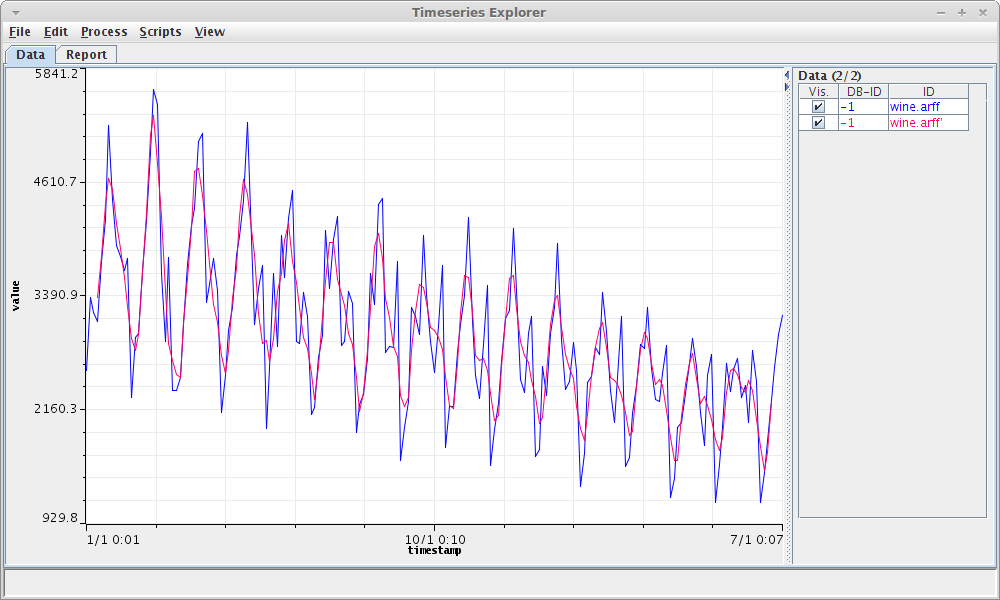
\includegraphics[width=10.0cm]{images/timeseries_explorer.png}
  \caption{Timeseries Explorer displaying wine sales, raw and smoothed with a Savitzky-Golay filter.}
  \label{timeseries_explorer}
\end{figure}

\section{Weka Explorer}
Using the \textit{Timeseries Forecasting} package\cite{wekatimeseries}, you 
can perform basic timeseries analysis in the Weka Explorer as well. The
\textit{Forecast} tab in the Explorer allows you to configure a forecaster, 
specifiying the attribute to forecast, what periodicity to use, etc. Figure
\ref{weka-timeseries} shows a screenshot of a forecast for Australian wine
sales of fortified wine. An overall downward trend, despite seasonal ups and 
downs, is clearly visible.

\begin{figure}[htb]
  \centering
  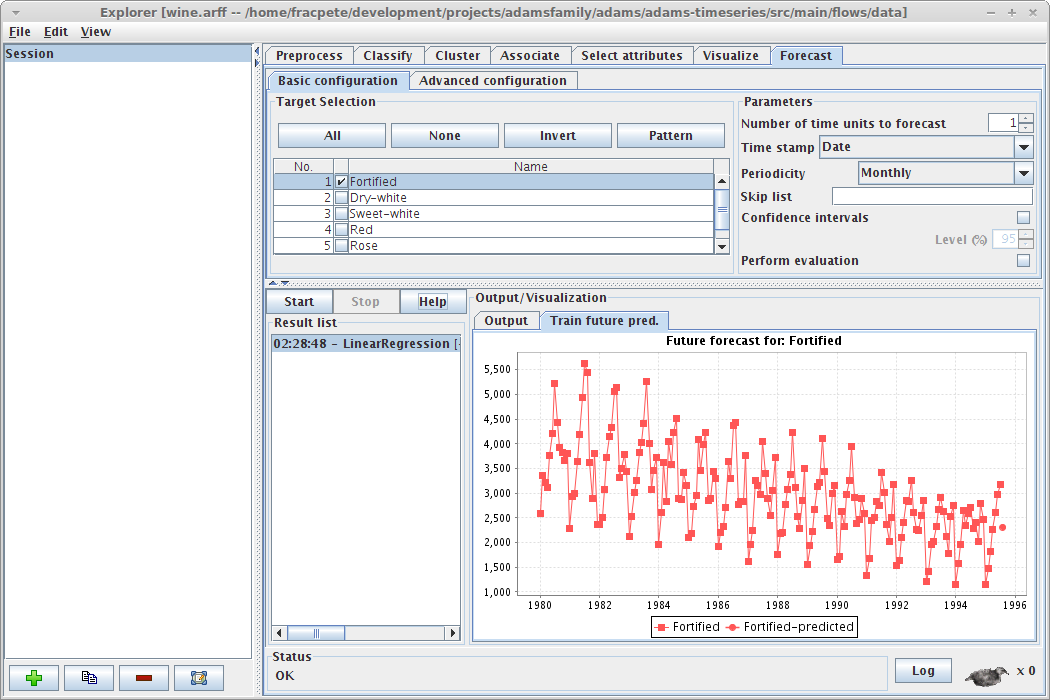
\includegraphics[width=10.0cm]{images/weka-timeseries.png}
  \caption{WEKA Explorer displaying forecasts for Australian wine sales.}
  \label{weka-timeseries}
\end{figure}

%%%%%%%%%%%%%%%%%%%%%%%%%%%%%%%%%%%
\chapter{Setup}
The following properties file contains the default format strings for
periodicity types:
\begin{verbatim}
  adams/data/timeseries/Periodicity.props
\end{verbatim}

%%%%%%%%%%%%%%%%%%%%%%%%%%%%%%%%%%%
% Copyright (c) 2009-2012 by the University of Waikato, Hamilton, NZ. 
% This work is made available under the terms of the 
% Creative Commons Attribution-ShareAlike 4.0 license,
% http://creativecommons.org/licenses/by-sa/4.0/.
%
% Version: $Revision$

\begin{thebibliography}{999}
	% to make the bibliography appear in the TOC
	\addcontentsline{toc}{chapter}{Bibliography}

    % references
	\bibitem{adams}
		\textit{ADAMS} -- Advanced Data mining and Machine learning System \\
		\url{https://adams.cms.waikato.ac.nz/}{}

	\bibitem{esrigrid}
	 	\textit{Esri Grid} -- a raster GIS file format deveoped by Esri. \\
		\url{https://en.wikipedia.org/wiki/Esri\_grid}{}

	\bibitem{kml}
	 	\textit{Keyhole Markup Language} -- an XML notation for expressing
	 	geographic annotation and visualization within Internet-based,
	 	two-dimensional maps and three-dimensional Earth browsers. \\
		\url{http://en.wikipedia.org/wiki/Keyhole\_Markup\_Language}{}

	\bibitem{postgresql}
	 	\textit{PostgreSQL} -- a powerful, open source object-relational
	 	database system. \\
		\url{http://www.postgresql.org/}{}

	\bibitem{postgis}
		\textit{PostGIS} -- a spatial database extender for PostgreSQL
		object-relational database. It adds support for geographic
		objects allowing location queries to be run in SQL.  \\
		\url{http://postgis.net/}{}

	\bibitem{srid4269}
	 	\textit{SRID 4269} -- or NAD 83 (North American Datum). \\
		\url{http://spatialreference.org/ref/epsg/4269/}{}

	\bibitem{mysql}
		\textit{MySQL} -- an open-source relational database management
		system (RDBMS) \\
		\url{http://www.mysql.com/}{}

\end{thebibliography}


\end{document}
